\documentclass{beamer} %
\usetheme{Dresden}
\usecolortheme{beaver}
\usepackage[brazil]{babel}
\usepackage[utf8x]{inputenc}
\usefonttheme{professionalfonts}
\usepackage{times}
\usepackage{graphicx}
\usepackage{tikz}
\usepackage{amsmath}
\usepackage{tabulary}
\usepackage{pgfgantt}
\usepackage{verbatim}
\usetikzlibrary{arrows,shapes}
\usepackage{adjustbox}
\usepackage{soul}
\usepackage{listings}
\usepackage{adjustbox}
\setbeamertemplate{itemize item}{\color{red}$\blacksquare$}
\usepackage{hyperref}
\title{MATRIX PROJECT}

\title{MATRIX PROJECT}
\institute{}
\author{EE1390}

\date{INTRODUCTION TO AI AND ML}

\begin{document}
\tikzstyle{every picture}+=[remember picture]
\lstset{language=C++}   
\everymath{\displaystyle}

\begin{frame}

	\titlepage
\end{frame}

%------------------------------------------------------


\begin{frame}{QUESTION - 20 }
\newline{\bf (IN GEOMETRIC FORM)}

Let K be an integer such that the triangle with vertices A = (k,-3k) ; B = (5,k) ; C = (-k,2) has area 28.Find the orthocentre of this triangle.



\begin{columns}

\column{0.6\textwidth}



\end{columns}

\end{frame}


\begin{frame}{QUESTION-20}

{\bf (IN MATRIX FORM)}  
Let k be an integer such that the triangle with vertices
\newline
\[
A = \begin{bmatrix}
k \\
-3k
\end{bmatrix},
B = \begin{bmatrix}
5 \\
k \end{bmatrix},
C = \begin{bmatrix}
-k \\
2 \end{bmatrix}\]
\newline
has area 28.Find the orthocentre of the triangle.
\end{frame}

\begin{frame}{SOLUTION:}

{ Vertices :}
\newline
\[
A = \begin{bmatrix}
k \\
-3k
\end{bmatrix},
B = \begin{bmatrix}
5 \\
k \end{bmatrix},
C = \begin{bmatrix}
-k \\
2 \end{bmatrix}\]
\newline { area} = 28



\end{frame}
\begin{frame}
Area of the triangle in matrix form:
\newline

\centering
\begin{vmatrix}k & 5 & -k\\
-3k & k & 2\\
1 & 1 & 1\end{vmatrix} $=$ 56
\newline

$|$ $k(k - 2)$ $-$ $5(-3k - 2)$ $-$ $ k(-3k - k)$ $|$ = 56
\end{frame}
\begin{frame}
CASE 1:
\newline

 $k(k-2)-5(-3k-2)-k(-3k-k)= 56$
 \newline
 
 $k^2-2k+15k+10+3k^2+k^2=56$
\newline

$5k^2+13k-46=0$
\newline

$k = 2, k = \frac{-23}{5}$
 \end{frame}

\begin{frame}
CASE 2:
\newline

$k(k-2)-5(-3k-2)-k(-3k-k) = -56$
\newline

$k^2-2k+15k+10+3k^2+k^2 = -56$
\newline

$5k^2+13k+66 = 0$
\newline

$k$ $is$ $complex$ $in$ $this$ $case.$ 
\end{frame}

\begin{frame}
Since k is given to be an integer,
\newline

\begin{center}
$k$ = $2$
\end{center}
\newline

On substituting the value of k in the given coordinates
\newline

\centering
A =\begin{bmatrix}
2\\
6\end{bmatrix},
B =\begin{bmatrix}
5\\
2\end{bmatrix},
C =\begin{bmatrix}
-2\\
2
\end{bmatrix}
\end{frame}

\begin{frame}{TO FIND THE ORTHOCENTER}
The point of intersection of altitudes is the orthocenter of the triangle.
\newline

Let D be the foot of perpendicular from A to BC,
\newline

The equation of AD is
\newline
\begin{center}
$(B - C)^T(X-A) = 0$
\end{center}
\newline
\begin{equation}
(B-C)^T(X) = (B - C)^T(A)
\end{equation}

\end{frame}

\begin{frame}
\newline

Let E be the foot of perpendicular from B to AC,
\newline

The equation of BE is
\newline
\begin{center}
$(C - A)^T(X-B) = 0$
\end{center}
\newline
\begin{equation}
(C - A)^T(X) = (C - A)^T(B)
\end{equation}

\end{frame}
\begin{frame}
The point of intersection of AD and BE(altitudes) is the orthocentre H.
\newline
\begin{equation}
{\begin{bmatrix}
B - C & C -A \end{bmatrix}}^TX = \begin{bmatrix} (B - C)^TA\\
(C-A)^TB\end{bmatrix}
\end{equation}
    $(B - C)$ =   \begin{bmatrix}
 5 \\
 2 \end{bmatrix} $-$ \begin{bmatrix}
-2\\
2\end{bmatrix} = \begin{bmatrix}
7\\
0\end{bmatrix}
\newline

$(B - C)^TA$ = \begin{bmatrix}
7 & 0 \\ \end{bmatrix}\begin{bmatrix}
2 \\
 -6 \end{bmatrix}= $14$
 \newline
 
  $(C - A)$ =   \begin{bmatrix}
 -2 \\
 2 \end{bmatrix} $-$ \begin{bmatrix}
2\\
-6\end{bmatrix} = \begin{bmatrix}
-4\\
8\end{bmatrix}
\newline

$(C - A)^TB$ = \begin{bmatrix}
-4 & 8 \\ \end{bmatrix}\begin{bmatrix}
5 \\
 2 \end{bmatrix}= $-4$
 

\end{frame}

\begin{frame}
Substituting the above values in equation (3),
\newline

{\begin{bmatrix} 7 & -4 \\
0 & 8 \end{bmatrix}}^T\begin{bmatrix}x\\ 
y\end{bmatrix} $=$ \begin{bmatrix}14 \\
-4 \end{bmatrix}
\newline

\begin{bmatrix}7 & 0\\
-4 & 8 \end{bmatrix}\begin{bmatrix}x\\
y\end{bmatrix} $=$ \begin{bmatrix}14 \\
-4 \end{bmatrix}
\newline

\begin{bmatrix}x \\
y \end{bmatrix} &=& {\begin{bmatrix}7 & 0\\
-4 & 8\end{bmatrix}}^{-1}
\begin{bmatrix}14\\
-4\end{bmatrix}
\newline

\begin{bmatrix}x \\
y \end{bmatrix} $=$ \begin{bmatrix}\frac{8}{56} & 0\\
\frac{4}{56} & \frac{7}{56}\end{bmatrix}\begin{bmatrix}14\\
-4\end{bmatrix} $=$ \begin{bmatrix}\frac{112}{56}\\
\frac{28}{56} \end{bmatrix} $=$ \begin{bmatrix}2\\
0.5\end{bmatrix}
 \end{frame}
\begin{frame}

\begin{tikzpicture}[scale = 0.5]
      \draw[->] (-3,0) -- (5,0) node[right] {$x$};
      \draw[->] (0,-6) -- (0,4) node[above] {$y$};
      \draw (2,-6) -- (5,2):
      \draw (2,-6) -- (-2,2):
      \draw (5, 2) -- (-2,2):
      \draw(2,-6) -- (2,2):
      \draw(5,2) -- (-0.6,-0.8):
      \locate (2,0.5)
    \end{tikzpicture}
    \newline
    
    Therefore,the orthocenter of the triangle is (2,0.5)
\end{frame}
\begin{frame}
\begin{figure}[h]
\begin{center}
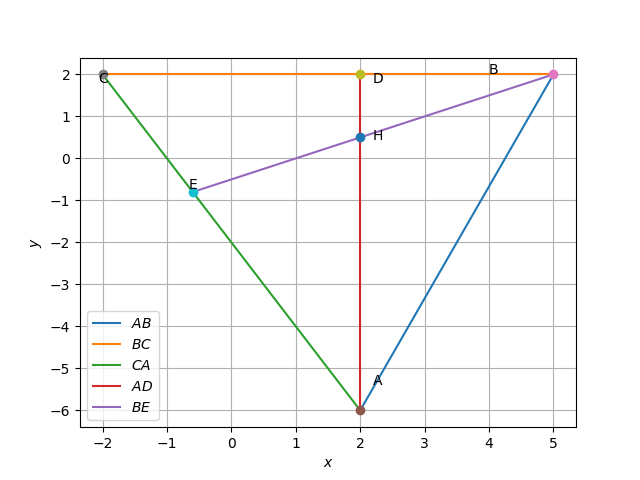
\includegraphics[scale = 0.6]{orthocentre.png}
\end{figure}
\end{center}
\end{frame}
\begin{frame}
   \huge $ Presented$ $by$
    \newline
    \begin{center}
    \bf { \begin{matrix} Tejaswini \\ and\\ Varuni\end{matrix}}
    \end{center}
\end{frame}
\end{document}
